\chapter{Introduction}

\section{Motivation}
\label{sec:motivation}

Cities are full of players, each with different interests. Citizens want to maximize their quality of life, which usually means living in spacious homes, in peaceful places, full of nature, but still having access to employment opportunities, leisure, health, education, among others. Real estate agents and construction companies want to build buildings, houses and condominiums that maximize their profits, choosing the locations with the highest demand and lowest costs. Land and property owners seek to buy cheap assets with the expectation that they will appreciate in value in the future or extract rental income.

However, the dynamics of cities are shaped by countless conflicts of interest, many of which are antagonistic. It's impossible, for example, for everyone to live in contact with nature, since as each family builds its own house, the neighbor's nature diminishes. Thus, there are two ways of coexisting in space: through power relations, in which the most powerful agent has its interest served (or negotiated) to the detriment of another, or a central planner mediates this conflict in order to generate the most favorable outcome for everyone.

The main institution responsible for mediating conflicts in the urban sphere of São Paulo, the most populous city in the Americas, is the Strategic Master Plan (SMP). The SMP is a municipal law that establishes city rules such as zoning and regulations on building standards. The 2014 master plan brought significant changes compared to its 2002 predecessor, and is internationally recognized for its approach to combating inequalities and encouraging the use of public transport.

While the 2002 plan decentralized much of the zoning decisions to the subprefectures, the 2014 SMP followed a modern approach, in line with the urbanism literature of \textit{Transit Oriented Development} (TOD). Previously, each sub-prefecture had a leading role in the zoning of its region, while in the new plan, regulation was defined at the municipal level and centralized. The old system had great difficulty in dealing with conflicts of interest and local groups had the ability to contain densification in desirable areas\footnote{Movement known as \textit{Not in My Backyard} (NIMBY)}, harming the sustainable development of the city.

The TOD literature, which emerged in the late 1980s but only became popular after the 2000s, advocates mobility as one of the main pillars of city development \cite{Ibraeva2020}. The TOD proposal is to bring families closer to opportunities by directing urban development around high-capacity public transport infrastructure, leading to improved mobility and greater densification. This reduces dependence on individual motorized transport, which generates negative externalities.

The ideas of the TOD not only influence the 2014 SMP, but are a structural part of it. Among the stated objectives of the master plan, the first four stand out:

{\small
\begin{quote}
    Art. 7 The Urban Development Policy
    and the Strategic Master Plan are guided by the
    following strategic objectives:

    I - contain the process of horizontal expansion of the urban agglomeration, helping to preserve the metropolitan green belt;

    II - accommodate urban growth in underutilized areas equipped with infrastructure and around the high and medium capacity public transport network

    III - reduce the need to commute, balancing the relationship between places of employment and places of residence;

    IV - expand high and medium capacity public transport networks and non-motorized modes, rationalizing the use of automobiles;
\end{quote}
}
Having said that, the question motivating this research is whether, 10 years after the master plan came into force, it is possible to identify whether it is fulfilling its objectives - in particular, the objective of densifying areas close to public transport infrastructure.

\section{Strategic Master Plan (SMP)}
\label{sec:master-plan}

This section is dedicated to understanding which tools are available to the master plan to achieve its objectives \cite{PDE2002, PDE2014, PDE2023}. However, the SMP has several instruments that act not only on new buildings, but also on the requalification of already built plots. The focus of this research is on the three main instruments designed to regulate new constructions. These are the floor area ratio, the land quota and the hight limit. Other instruments, although important, do not aim to regulate the population density of each area.

The SMP divided the city map into macro-areas, macro-zones and special zones, each with specific objectives and respective restrictions for each instrument. It also created a special regime for plots close to high-capacity public transport infrastructure, a region called Urban Transformation Structuring Axes (in Portuguese, Eixos de Estruturação da Transformação Urbana) or simply axis.

\subsection*{Structuring Axes of Urban Transformation}

The axes are defined by their proximity to high-capacity public transport, and in São Paulo this activation occurs in two ways. The first is through train, metro or monorail stations, which create an area of influence with a radius of 400 meters around the access points. The second is through municipal and intercity bus corridors, which create an area of influence of 150 meters on each side of the road along the corridor.

In the axis zones, in addition to a special regime for the three instruments that will be presented, other measures are implemented to encourage the use of public transport. For example, to discourage the use of cars, restrictions have been placed on the number of parking spaces, which were previously encouraged by the 2002 SMP. Thus, the axes become test areas for the effectiveness of these instruments, as they are applied to their full potential.

\subsection*{Floor Area Ratio (FAR)}

The floor area ratio (FAR) is an instrument used worldwide\footnote{Floor Area Ratio} (FAR) or \textit{Floor Area Ratio} in master plans to regulate \textbf{building density}. The FAR determines how many times the area of the plot can be built on. São Paulo's legislation prescribes a basic floor area ratio of 1 in the property rights of all plots in the city, meaning that it is permissible to build once the area of the plot. If an owner wants to build 4 floors on his plot, with a FAR of 1, he can only occupy 1/4 of the land area. From the point of view of the law, the potential to build more than one square meter over the area of the plot is not included in the right of ownership, and therefore belongs to society, not to the owner of the plot.

In each macro-area of the city there are different restrictions for the minimum and maximum FAR - the basic one remains 1 throughout the city. In the Urban Structuring and Qualification Macrozone, the minimum FAR varies between 0.3 and 0.5 depending on which macro-area it is in, and the maximum is always 2. In the Environmental Protection and Recovery Macrozone, there is no minimum FAR and the maximum FAR varies between 0.1 and 1, depending on the level of protection that has been assigned to the region. In these preservation areas, other regulations may also apply\footnote{The relevant state legislation applies, especially the specific laws for the Billings and Guarapiranga Basins}.

When the region is activated by high-capacity public transport, there are modifiers on the FAR . In the Urban Structuring and Qualification Macrozone, if there is an axis region, the maximum FAR increases to 4. In the Environmental Protection and Recovery Macrozone, as long as the area is outside the source protection region, the maximum FAR becomes 2. In this way, the SMP allows double the building density around transport infrastructure, demonstrating its commitment to TOD.

\subsection*{Hight Limit}

Hight limit is also a common instrument regulated in master plans to control verticalization in the city. Hight limit, among the instruments discussed, is the most visible to the eye of people passing by on the street or from the air, when arriving by plane at Guarulhos or Congonhas airport. In the Urban Structuring and Qualification Macrozone, the maximum height is 28m or, in terms of floors, the first floor plus 8 floors. In the Environmental Protection and Recovery Macrozone areas, the maximum height is 15m, or the first floor plus 4 floors.

As a way of encouraging real estate production in the axes, in the Urban Structuring and Qualification Macrozone there is no limit on the height of buildings, which are limited only by the FAR . The axes in the Environmental Protection and Recovery Macrozone have a maximum height limit of 28m.

An important detail is that there is an identity between FAR , verticalization and occupancy rate. The occupancy rate is the percentage of the land area that is built on. For example, on a plot of land with a FAR of 4, if 8 floors are to be built, the occupancy rate must be 50\%. Similarly, if the occupancy rate is set at 100\%, for example, the number of floors must be 4. More details on this discussion, as well as a comparison between building density and verticalization, can be found in Appendix \ref{appendix:verticalization}.

\subsection*{Land Quota}

The quota share, on the other hand, is not a common instrument to see in master plans and can be considered a relatively experimental measure - unlike the FAR and hight limit, which are consolidated instruments. This instrument is responsible for regulating housing density. Knowing the land quota ($Q$) and the area of the plot ($A_t$), it is possible to identify the minimum number of housing units ($N_{min}$) that the plot must have, following Equation \ref{eq:cotaparte} below.

\begin{equation}
    N_{min} = \frac{\text{CA}_{\text{used}}}{\text{CA}_{max}}\cdot \frac{A_t}{Q}
    \label{eq:cotaparte}
\end{equation}


On a plot of 1000 $m^2$ with a share of 20, if the maximum FAR is used, at least 50 housing units must be built. However, this doesn't mean that each unit will be 20$m^2$, but this will be the average height of the plot that each unit occupies. The size of each unit will be the land quota times the FAR used, i.e. if the FAR is equal to four in the example given, the units will average 80$m^2$, which could also mean half the units with 40$m^2$ and the other half with 120$m^2$. In this sense, it's worth noting that although a larger FAR in the batch doesn't increase the minimum number of units to be produced, it does allow the minimum units to be more spacious. Furthermore, when the FAR used is lower than the maximum, the minimum number of units to be provided also decreases.

The quota share, however, is not an instrument applicable to the whole city, but only to the axis region, where it is 20 in the Urban Structuring and Qualification Macrozone and 40 in the Environmental Protection and Recovery Macrozone.

\section{The problem}
\label{sec:problem}

In order to assess whether the SMP has actually succeeded in meeting its objectives, three questions need to be answered. The diagram in Figure \ref{fig:diagram} helps to understand each of them.

\begin{figure}[h]
    \caption{From the regulatory instruments to the expected result}
    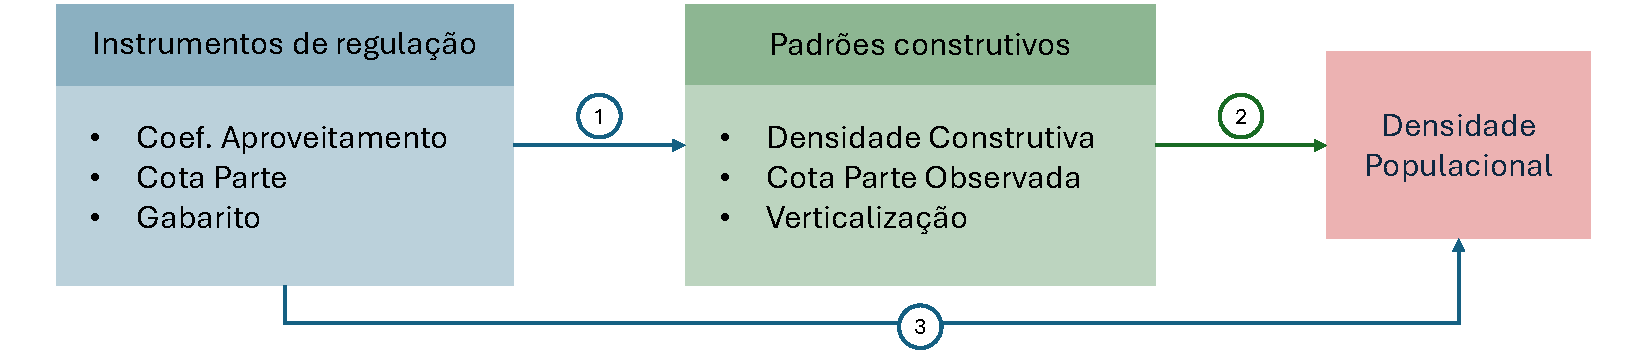
\includegraphics[width = \linewidth]{figuras/desenho_proposta.pdf}
    \label{fig:diagram}
\end{figure}

\subsection*{Has regulation been able to influence building standards in the city in the way expected?}

Through the instruments presented in Section \ref{sec:master-plan}, the SMP intended real estate development to be concentrated in the Urban Structuring and Qualification Macrozone, especially in the axis, which received a new set of rules. To a large extent, these changes allowed for greater building density, unlimited verticalization and imposed a minimum housing density. However, as mentioned in Section \ref{sec:motivation}, the city is made up of various interests, and the real estate market is a central player in this respect.

The real estate market, which is responsible for actually building new housing, responds to regulation by always seeking to maximize its profits. As the regulation didn't create incentives and in fact only changed permissions in each region of the city, the real estate market doesn't necessarily accept the new set of rules as an invitation to build the typology that the SMP wants to see in the axis. Within the limits of the FAR legislation of between 2 and 4, there is a lot of freedom for the market to choose what to build. Furthermore, there is always the option of not building in these areas, when the benefit of greater building potential is not enough to offset the tax that comes from exceeding the basic FAR .

\subsection*{Are regulated and incentivized building standards really capable of generating the expected density?}

In other words, is it possible to say that higher building density, more verticalization and higher housing density translate into higher population density? Although the question is simple, there are nuances to consider. Firstly, it is essential to determine whether these three components of the building pattern are relevant and which of them has the greatest influence on population density.

If building density is a determining factor in population density, the FAR instrument becomes important. Similarly, if housing density or verticalization are more prominent, the land quota and the hight limit become relevant. Thus, answering this question helps to identify which of the instruments analyzed in question 1 are most significant.

\subsection*{Has regulation been able to influence population density in the city?}

The SMP proposed a causal relationship, illustrated in Figure \ref{fig:diagram}, which assumes that if the first two conditions are met, the increase in population density will be a direct consequence. In other words, the third question would become unnecessary if the first two were confirmed.

However, this relationship is not guaranteed, as other factors can also influence population density, regardless of the regulations introduced. It is therefore essential to assess the total effect of regulation on population density in order to understand the full and real impact of the policies implemented.

\subsection*{Direction in article}

Chapter \ref{chp:review} presents a brief literature review. Chapter \ref{chp:data} presents the data used in the analysis. Chapter \ref{chp:analysis} discusses the methodology and results for each of the questions. In Chapter \ref{chp:conclusion} the final reflections are presented, in Section \ref{sec:conclusion} the focus is on the main results, and in \ref{sec:contributions} a discussion is made with more direct implications for the public debate. Finally, in the Appendices there are discussions of important details, but which are tangential to the narrative of the work.

The codes used to generate the results presented are publicly available for verification, replication or use for other purposes, provided that this work is cited appropriately\footnote{The code can be accessed on the GitHub page \href{https://github.com/gustavo-tm}{at this link.}}.


\chapter{Literary Review}
\label{chp:review}

\section{The role of regulation}

In microeconomic literature there are various models that try to understand the economic dynamics of the city, analyzing how market forces act in the absence of regulation. Using formal assumptions and mathematical proofs, it is possible to solve the models for some endogenous variables, such as price per square meter in the city, land use, population density, among others. What these models generally have in common is that if the market is treated \textit{laissez-faire}\footnote{The \textit{laissez-faire} treatment refers to the government's having little influence on the decisions of economic agents}, there will be greater densification in the center, where there is a supply of jobs. When there are multiple centers, or high-capacity public transport hubs, there is also greater densification around them \cite{papageorgiou2012essay, fujita1989urban}.


This is because densification brings various economic benefits. Technological agglomeration $(i)$ increases worker productivity, as jobs are more concentrated and there is a "spillover" of knowledge between firms in the region. In addition, a larger and more diverse supply of labor leads to greater competitiveness and efficiency in choosing the right person for each job. Pecuniary agglomeration $(ii)$ reduce firms' costs without altering their productivity. With greater demand for services such as security, cleaning, contracting and advocacy, these markets develop, become more competitive, efficient and cheaper. There are even specialized niche services, which may only be available and accessible in large urban centers. Retail agglomeration $(iii)$ brings gains for consumers and traders. When retailers are agglomerated, consumers can choose from more options and travel less between destinations if they want to buy more than one item. In this way, consumers gain and so do traders, since with more consumers and greater flow, sales increase. Finally, the cost of transportation $(iv)$ is one of the factors that changes the most when there is density. The reduction in transportation costs, which can be considered a pecuniary agglomeration economy, occurs not only for workers, who travel less to job opportunities, but also for firms that spend less on transporting their goods and services \cite{brueckner2011lectures}.

However, by introducing market failures into these models, the organization of the city in the absence of regulation can be associated with undesirable scenarios. These market failures often lead to an expansion of the urban sprawl, with negative implications for the environment, as well as a loss of the benefits of agglomeration. One example of a market failure is related to car traffic. This means of individual motorized transport reduces the costs of long journeys, enabling citizens to live further away from their destinations. However, as well as expanding the urban sprawl, introducing a risk of accidents and emitting pollutants, every extra car on the road slows down everyone else's journey. Although these harms are negligible when it comes to individual choices about whether or not to use a car - in other words, a rational individual is not going to stop using a car - in a city with millions of inhabitants, the negligible individual cost of each car adds up to have a significant impact on society.

In this sense, the government could intervene to correct these market failures, for example by introducing an urban toll. In this way, the negative externalities of this individual choice to use a car would be internalized. With the money collected from this tax, the damage caused could be compensated for through public investment. However, such a measure is difficult to implement, leading decision-makers to take another route to combat externalities. Regulating building standards could be an alternative way of dealing with the problem, preventing externalities from occurring. On this front, the FAR is a widely used instrument for regulating building standards and is included in the master plans of modern cities in the United States, Canada, Germany, France, etc.

\begin{figure}[h]
    \caption{Impact of regulation on the city's FAR}
    \centering
    \begin{subfigure}{.6\linewidth}
        \begin{tikzpicture}

    \begin{axis}[standard,
        xtick={0},
        ytick={.5},
        xticklabels = {},
        yticklabels = {$FAR_{reg}$},
        samples=100,
        xlabel={Distance to center ($x$)},
        ylabel={FAR},
        xmin=0,xmax=2,
        ymin=.2,ymax=1,
        y label style={anchor=east},
        x label style={anchor=north},
        clip=false
    ]
    
\addplot[domain={0:2}]{.8*e^(-.9*x)+.1} node[pos=1] (point1) {};
\node [right] at (point1) {\textit{laissez-faire}};

\addplot[domain={(ln(4.8)/1.3):2}]{1.2*e^(-1.3*x)+.25} node[pos=1] (point2) {};
\node [right] at (point2) {regulado};

\addplot[domain={0:(ln(4.8)/1.3)}]{.5};

\addplot[black, dashed] coordinates {((ln(4.8)/1.3),0) ((ln(4.8)/1.3),.5)};

\end{axis}
\end{tikzpicture}
    \end{subfigure}
    \label{fig:FAR}
\end{figure}

If the maximum regulated FAR is higher than the market demand, the observed FAR will be lower than the limit, i.e. the regulation does not impact that region directly. In regions where the demand for housing is higher than permitted, part of the demand needs to be relocated territorially so that the limit is not exceeded. In the case of the 2014 SMP, the idea is to limit densification in peripheral and environmentally protected regions, directing densification towards the central regions. However, if the excess demand is in a central area, it will spread to the outskirts, causing the opposite effect to that stipulated. In Figure \ref{fig:FAR} you can see an example of the maximum FAR in the city as a whole and the excess demand for housing in the center, which with the maximum limit in FAR, disperses into more distant territories.


Therefore, if the central planner incorrectly identifies the market demand in each region of the city, it is possible that the repressed demand will trigger a process of expansion of the urban sprawl and all the negative externalities discussed above. Furthermore, when regulation is too restrictive, there is an indirect incentive for an informal market to develop. In this sense, although FAR is a powerful tool in the urban planner's arsenal, it is also dangerous, as it can lead to adverse effects.

\section{Existing evidences about the SMP 2014}

The literature on the impact of São Paulo's Strategic Master Plan (SMP), especially with regard to increasing density near public transportation, is limited, with little quantitative production focused on causal inference. Most of the existing studies have a descriptive or discussion profile, observing effects without establishing clear causal relationships. The revision of the SMP between 2021 and 2023 generated a series of publications, many of them descriptive, which discuss the changes introduced, but there is still a gap in studies that use quantitative methods to assess the real impact of these policies.

During the SMP review period, several technical notes were important for the discussions that were taking place. There was evidence that pointed to a densification of construction in the axis regions, even though there was spatial heterogeneity \cite{IU50, nt1, nt2, Marques2023}. Some statistics were also done to analyze economic activity and formal employment \cite{IU52, IU54}.

The main study that stands out for presenting causal inference for the increase in building density was entitled ``Estimating the economic value of zoning reform''. The article shows that in regions where there has been an increase in the maximum FAR, an increase in building density can be observed in relation to those that have maintained the same, or reduced the maximum FAR \cite{Anagol2021}.

However, there is a gap in the literature when it comes to identifying the effect of SMP on population density. The descriptive statistics generated were largely inconclusive about the effectiveness of the SMP \cite{IU51, IU66}. Also, in the document released in 2021 with the diagnosis of the developments of the SMP made by the Municipal Department of Urbanism and Licensing of the city of São Paulo, the following conclusion about the effectiveness of the axes stands out: ``After the analyses carried out by the monitoring, it is possible to verify that there has been great construction densification in some areas of the city, but there are still no conditions to measure
population density'' \cite{PDE:diagnostico}.



\chapter{Data}
\label{chp:data}

\section{Building Standards}
\label{sec:dadosIPTU}

As for the data on real estate developments, the IPTU database was chosen. For the purposes of this article, it is the most complete, since it doesn't represent a flow of new properties built every year like Embraesp's database, but it does present a real estate stock of everything that has already been built for formal housing in the city. That said, the 3,096,719 unique taxpayer numbers are registered, which, according to the definition of the data documentation in GeoSampa, ``Each urban property will correspond to an inscription number in the Tax Real Estate Register, understanding as property: I - the area of land, built or not, defined in the registration of the competent Real Estate Registry Service or in transcripts still in force''. The only data that doesn't appear on this database relates to irregular or unregistered plots - this topic will be discussed below.

Among the IPTU data available are the land area, the built-up area, the occupied area, the type of use and the number of floors in the development. With this data, it is possible to identify building standards in the city, keeping the calculations as faithful as possible to the way they are calculated by the regulations. Building density, for example, is defined by the FAR observed on the plot.

\begin{figure}[h]
    \centering
    \caption{Distribution of construction standards in each residential lot in São Paulo}
    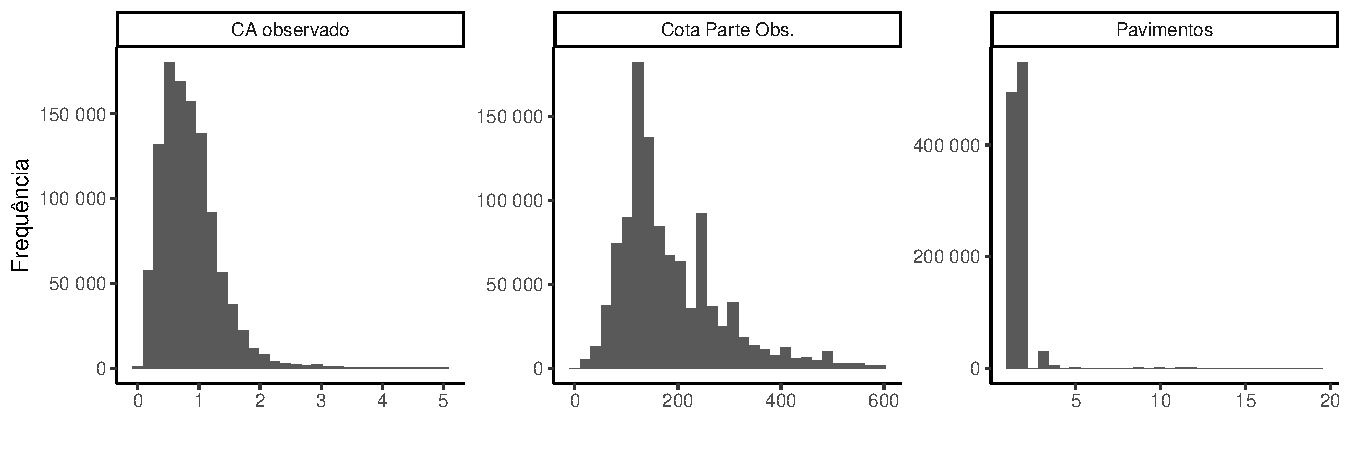
\includegraphics[width = \linewidth]{figuras/indicadores.pdf}
    \label{fig:histograms}
\end{figure}

In fact, if you look at the indicators in Figure \ref{fig:histograms}, you can see that São Paulo's housing profile is quite horizontal. It is surprising that 95\% of formal residential lots in São Paulo have 2 or fewer floors. In addition, the median FAR observed is 0.8, which indicates that more than half of the city's plots have been built on less than the area of the land. In addition, the median of the observed quota share of the city's plots is 155$m^2$, which represents a use of the land for a few housing units on average - the median quota share observed is approximately 8 times higher than the maximum quota share allowed in the axis. Despite this, from the 2000s onwards these indicators showed a trend towards densification and verticalization. Figure \ref{fig:indicadores-tempo} in Appendix \ref{appendix:figures} shows the evolution of construction patterns over time and Figure \ref{fig:area_construida} shows the distribution of built-up area dedicated to each type of use and density profile.

\section{Regulation}
\label{sec:dataSMP}

The regulation data is also publicly available on the city's website along with the SMP, but can also be accessed through GeoSampa. The main data used was the areas of influence of the axis activators, so that each region could be classified as inside or outside the axis zone.

\section{Population density}
\label{sec:dataCensus}

Population density data is produced by the IBGE demographic census, which takes place every 10 years. The 2020 Census was delayed until 2022 due to the pandemic and the data began to be released in 2024. So far, what has been made publicly available is the preliminary Census mesh. Given that the SMP came into force in 2014, the 2010 Census was used as a pre-SMP period and the 2022 Census as a post-SMP period. According to the 2022 survey, the current population of the city of São Paulo is 11,451,999, divided into 4,996,529 households, of which only 4,316,336 are occupied. Figure \ref{fig:population} shows the densest areas of the city. These include the city center (Sé) and the Paraisópolis and Heliópolis favelas.

\begin{figure}[!h]
    \centering
    \caption{Population density in São Paulo by census tract (Census 2022)}
    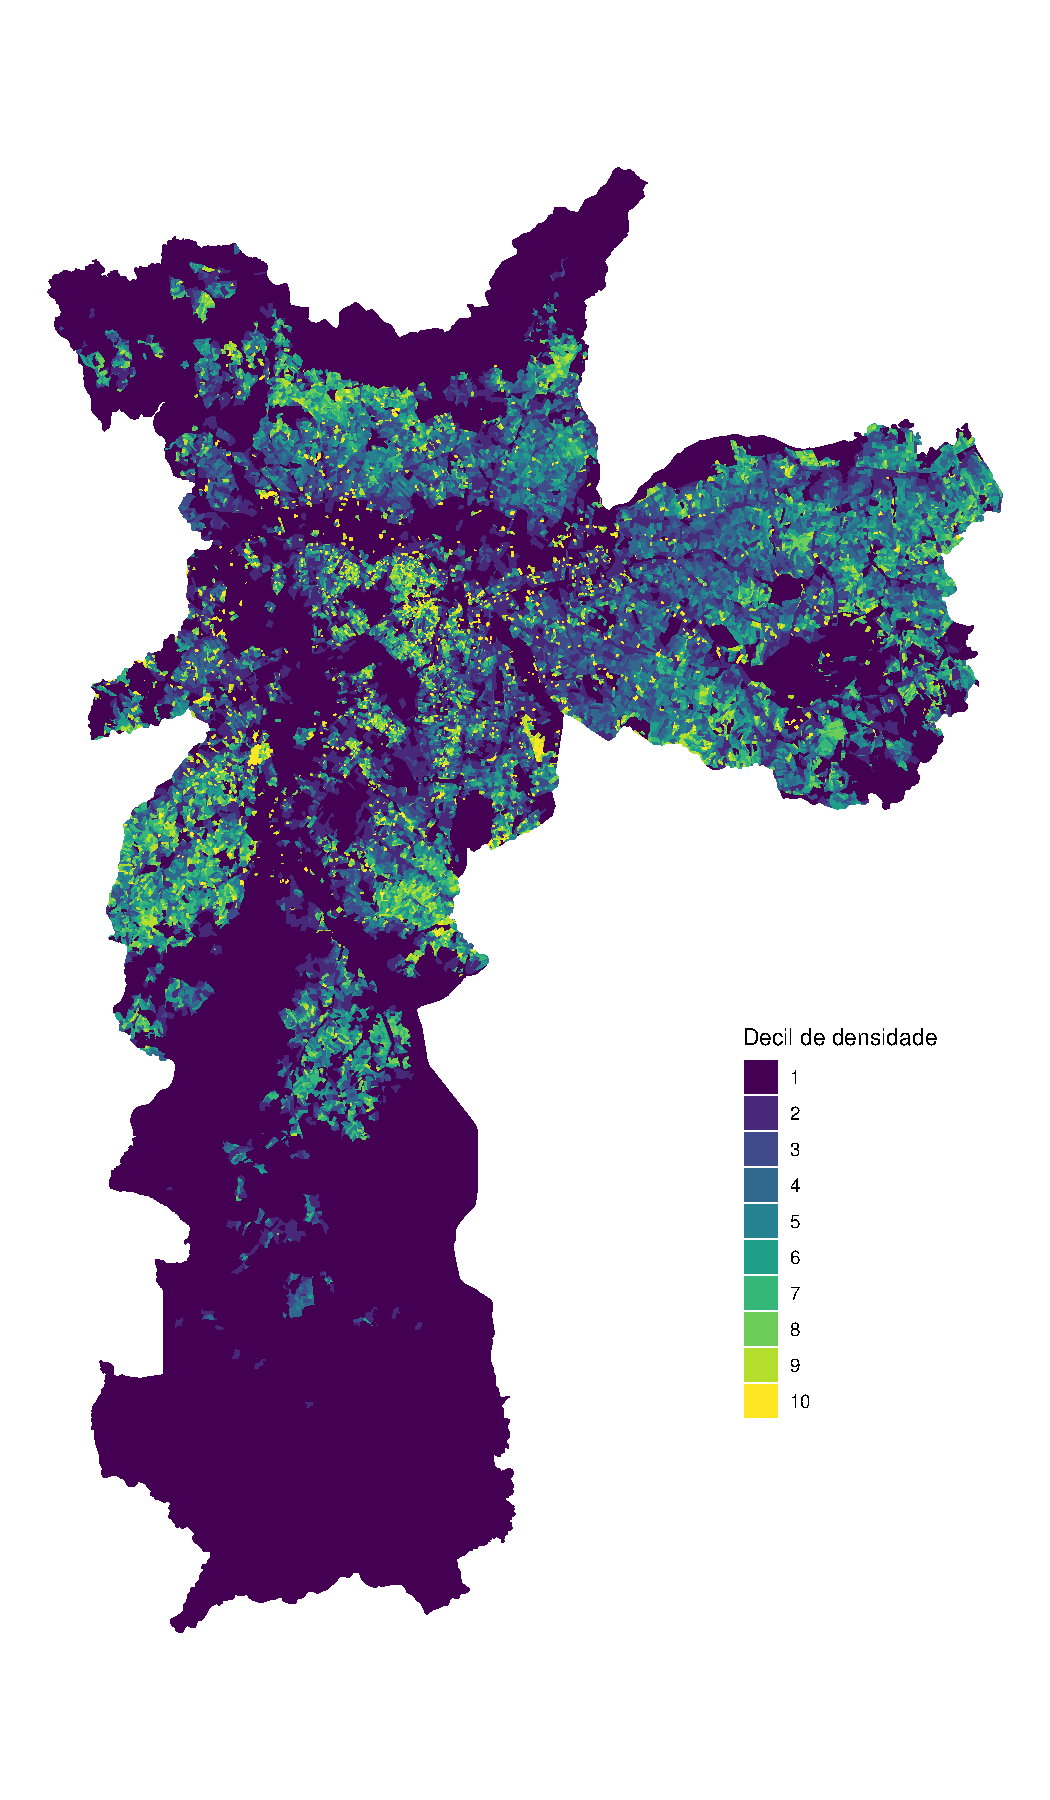
\includegraphics[width = .95\linewidth]{figuras/mapa-densidade.pdf}
    \label{fig:population}
\end{figure}

The closest unit of observation in the census that can be georeferenced is the census sector\footnote{In order to comply with the General Data Protection Law (LGPD), it is important to protect the anonymity of respondents, so there must be some kind of geographical aggregation}. The boundaries of the sectors are constructed in such a way that the census collection agent can cover the entire sector, minimizing measurement errors and optimizing the process. The methodology for delimiting census tracts takes into account various factors, such as elements in the landscape that constitute natural or artificial barriers and hinder the agent's work, stable and easily identifiable reference points on the ground, boundaries of territorial structures such as neighborhoods and blocks, among others \cite{IBGE2024}. A determining factor for the size of the census tract is the number of households to be interviewed, which in urbanized areas should be between 250 and 400 for the densest and between 150 and 250 for the least dense.

\clearpage
\section{Data Crossing}
\label{sec:dataCruz}

Part of the difficulty of discussing urban issues with data is the complexity of working with it. As can be seen in Table \ref{tab:datasets}, each database has a different level of observation and frequency. Therefore, some territorial and/or temporal aggregation is always necessary for analysis to be possible. As previously mentioned, the data processing methodology used in this article is available in a public repository.

\begin{table}[h!]
    \centering
    \caption{Information about each database}

    {\small
    \begin{tabular}{>{\raggedright\arraybackslash}p{0.125\linewidth} >{\raggedright\arraybackslash}p{0.50\linewidth} >{\centering\arraybackslash}p{0.125\linewidth} >{\raggedright\arraybackslash}p{0.15\linewidth}}
        % \toprule
        \textbf{Data} & \textbf{Source} & \textbf{Frequency} & \textbf{Scale} \\
        \midrule
        Census & Brazilian Institute of Geography and Statistics (IBGE) & Decennial & Census tract \\
        Property Tax (IPTU) & Property Tax and Maintenance Registry maintained by the Municipal Department of Finance (DECAD) of São Paulo's City Hall & Annual & Taxpayer \\
        Plots & Fiscal Real Estate Registry of the Municipal Department of Finance & Annual & Plot \\
        Regulation & Department of Urbanism and Licensing (SMUL) & 2014 & Zone perimeter \\
        \bottomrule
    \end{tabular}
    }
    \label{tab:datasets}
\end{table}


IPTU data is not georeferenced, so without other data it is not possible to cross-reference it with the Census. What makes this possible is that the unique IPTU taxpayer number is also the code of the Sector, Block and Lot (SQL) in which the development is located. In this sense, it is possible to break down the SQL and cross-reference it with the plot bases, which contain the geometry of each of the city's 1,677,980 plots. What explains the difference between the number of plots and the number of taxpayer numbers are the plots that contain a condominium, which can have several unique taxpayer numbers on just one plot. In the IPTU data, there are 1,314,353 taxpayers on lots with just one housing unit and 33,129 condominiums, which contain 1,782,366 units. When cross-referencing the IPTU SQL with the lots database, 44,319 taxpayers can't find a match in the other database, which represents a loss of 1.67\% of the units.

Regulation data is not coded with SQL, but it can be cross-referenced geographically. The zone perimeter is an administrative boundary generally equal to the blocks, but can be a subspace of the blocks in some cases. To determine which areas are densification axis, the axis zone perimeters were joined and an outline of the axis regions was created. The map with the result can be seen in Appendix \ref{appendix:figures}, Figure \ref{fig:eixos}.

As the zone perimeter is very much in line with the structure of the blocks, the classification of plots as being inside or outside the axis region is straightforward. Census sectors, on the other hand, follow a completely different structure. Sometimes a census tract contains several plots, but it is also possible for a plot to contain more than one census tract. For practical purposes, IPTU, census and regulation data have been geographically cross-referenced. A more detailed discussion can be found in Appendix \ref{appendix:cross-referencing}.

The census tracts are a partition\footnote{A partition is a division that occupies the entire space, with no intersection between the elements.} of the space of the city of São Paulo, which implies that the area of the census tract is made up not only of plots, but also of stretches containing streets, parks, non-residential uses, among other factors. Figure \ref{fig:area-sector} shows that only a third of the area of the census sector is dedicated to residential use. In addition, in the 1km radius of the axes, approximately 4\% of residential developments were built after the SMP\footnote{This figure is overestimated, since most of the buildings that were completed between 2014 and 2017 were approved during the 2002 SMP}.
 
\begin{figure}[h]
    \centering
    \caption{Dedication of census tract space for each use within a 1km radius of the axes}
    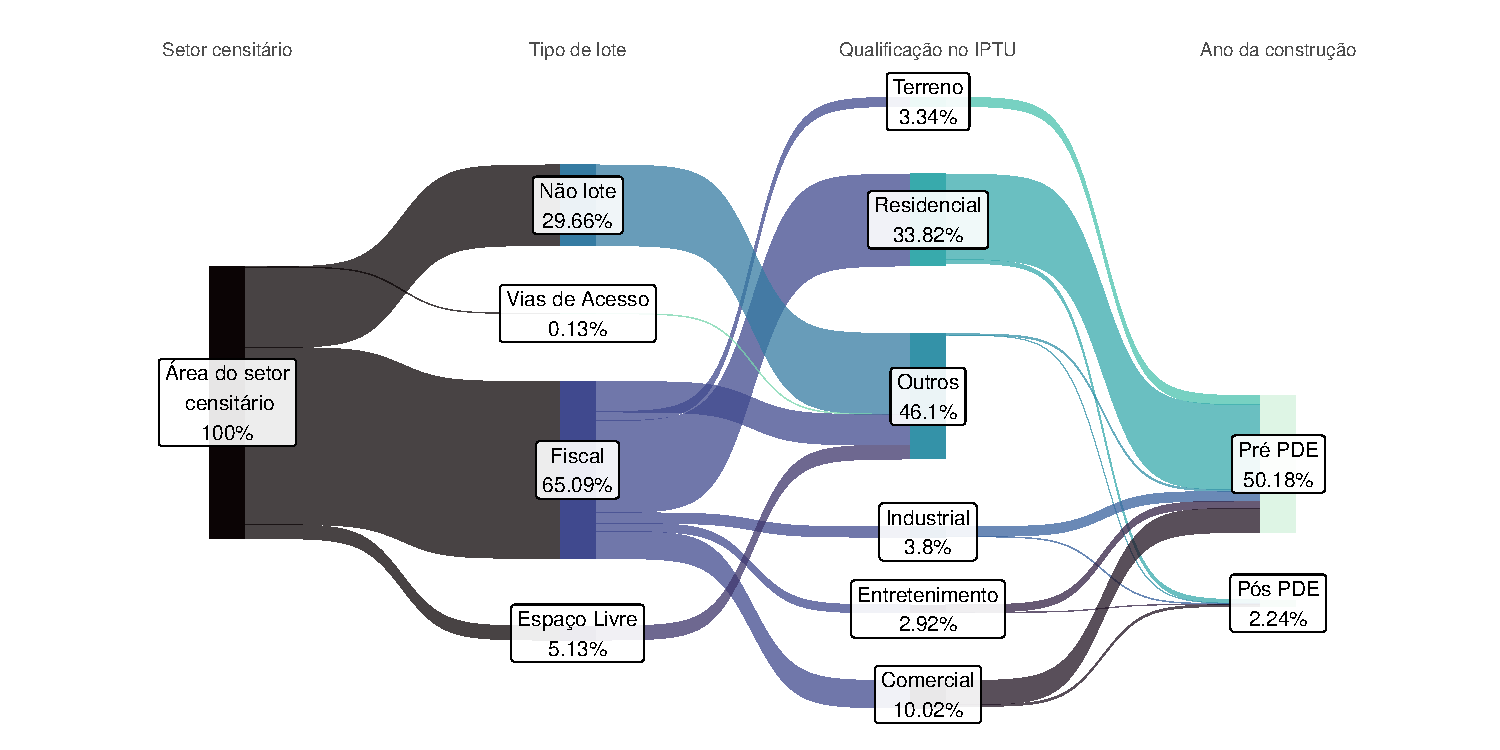
\includegraphics[width = \linewidth]{figuras/area_setor.pdf}
    \label{fig:area-sector}
\end{figure}

One opportunity when integrating this data is to validate information common to both. The number of dwellings, for example, is available in both the IPTU records and the Census. This comparison makes it possible to assess the level of informal housing in each region, since the Census offers more comprehensive and reliable data in this respect. Thus, a dwelling registered in the Census but missing from the IPTU can be considered informal. In quantitative terms, of the 4,996,529 households counted by the Census, only 2,641,635 are registered with the IPTU, which indicates a housing regularity index (legal) of approximately 52.87\%. More details on informality are discussed in Appendix \ref{appendix:informality}, but it is important to note that the results of this research apply exclusively to formal housing.



\chapter{Methodology and Results}
\label{chp:analysis}

As mentioned in Section \ref{sec:problem}, there are three questions to be answered, which can be seen in the diagram in Figure \ref{fig:diagram}. In the following sections, each of the questions will be answered through quantitative analysis of the data presented.


\section{From building pattern to population density}
\label{sec:perg1}


The aim of this section is to answer this question: \textbf{Are regulated and incentivized building standards actually capable of generating the expected density?} To this end, data from the 2022 Census and IPTU from the same year were considered. For this section, the regulation of each region of the city is not important, since the focus is on identifying the relationship between building density, housing density and sidewalks with population density and this relationship is not modified by the SMP. The influence of the SMP falls on these three components of the building pattern, through the regulation of the CA, land quota and hight limit, respectively. Thus, validating the importance of these building standards also means validating the regulatory instruments. Descriptive statistics can be found in Appendix \ref{appendix:neighborhoods}.

To infer the relationship between the 3 variables and population density, two complementary approaches were adopted and each has its strengths and weaknesses: linear regression (Section \ref{subsec:reglin}) and \textit{random forest} (Section \ref{subsec:randfor}). The main difference between the approaches is that regression, being in the world of econometrics, is more interpretable, but also requires certain assumptions to be valid. The \textit{random forest}, because it belongs to the world of \textit{machine learning}, has the characteristic of being more difficult to interpret, and is often considered a \textit{black box} model. On the other hand, while linear regression requires an economically based functional form, in the case of this section of the research, the regressors of population density are the regulatory instruments and not the economic factors discussed in Section \ref{chp:review} as distance to the center. This hinders the plausibility of exogeneity and the linear relationship between the instruments and population density, the \textit{random forest} finds the not necessarily linear relationships between the variables in the model on its own.


The first step in implementing these methodologies is to combine the databases at a single observation level. To keep the data at the most disaggregated scale possible, the data could be combined geographically at the census tract level. However, as discussed in Section \ref{sec:dataCensus}, the size of the census tract depends directly on both the population that inhabits it and its density, which would bias the regression\footnote{In this case, population density depends on the area of the census tract, which cannot be omitted from the regression. However, if it is used as a regressor, it will have a simultaneous relationship with the dependent variable, since the denser a region is, the smaller its area will be. Therefore, it would be necessary to estimate by simultaneous equations, making identification more complex, since there are not enough exogenous variables to recover the parameters of interest.} Therefore, the city map was cut into a grid with cells 800m wide and the data from both the census and the IPTU were aggregated on this scale. More technical details can be found in Appendix \ref{appendix:cross-referencing}.

Finally, only the raster cells with a low degree of informality were selected. The irregularity spectrum was calculated by comparing the number of households registered in the Census with the total number of units registered in the IPTU. When a region is at the extreme left of the spectrum (close to 0\%), this indicates that although there are households registered in the Census, the area does not have formal housing. Values close to 50\% reflect a balance between Census and IPTU data, indicating a lack of informality. Values above 50\%, which represent a higher number of units in the IPTU than in the Census, are rare. For more details on informality, see Appendix \ref{appendix:informality}.

\subsection{Linear regression approach}
\label{subsec:reglin}

{\tiny
\begin{table}[h]
\caption{Regression results for raster cells that present irregularity spectrum between 45 and 55\% in 2022} 
\centering
\fontsize{10.0pt}{12pt}\selectfont
\begin{tabular*}{.9\linewidth}{@{\extracolsep{\fill}}lcccc}
\toprule
 & \multicolumn{2}{c}{y = Population} & \multicolumn{2}{c}{y = Density} \\ 
\cmidrule(lr){2-3} \cmidrule(lr){4-5}
  & (A) Linear & (B) Log & (C) Linear & (D) Log \\ 
\midrule\addlinespace[2.5pt]
Intercept & 2121.210*** & 7.814*** & 6240.590*** & 8.583*** \\ 
Dwellings & 1.476*** & 0.000*** &  &  \\ 
Built area (m2) & 0.000 & 0.000+ &  &  \\ 
Verticalization & -131.656*** & -0.036** & 24.817 & -0.033 \\ 
Built Density &  &  & 705.142 & 0.199** \\ 
{Dwelling Unit Density} & {} & {} & {0.187***} & {0.000*} \\ 
\midrule
Num.Obs. & 332 & 332 & 332 & 332 \\ 
R2 & 0.861 & 0.602 & 0.319 & 0.223 \\ 
R2 Adj. & 0.860 & 0.598 & 0.313 & 0.216 \\ 
\bottomrule\vspace{0pt}
\end{tabular*}
\label{tab:regressao-1}
\begin{minipage}{.9\linewidth}
+ p < 0.1, * p < 0.05, ** p < 0.01, *** p < 0.001\\
\end{minipage}
\end{table}


}

Table \ref{tab:regressao-1} shows the results of four regressions, all with the same purpose, but with different functional forms. In the first two columns, the population is regressed in units, square meters of built area and an indicator of verticalization. Interpreting the first column (A), it is possible to infer that if the other components remain constant, one more housing unit is associated with 1.47 more residents in the region. The number of square meters built is not statistically significant. The verticalization coefficient indicates that an increase of 1 in verticalization\footnote{An increase of 1 in verticalization would imply that all the buildings in the \textit{raster} cell had an extra floor} on average is associated with 130 fewer people in the \textit{raster} cell. For comparison, the average population per cell is 4,600 inhabitants, with considerable dispersion. The distribution of the \textit{rasters} population can be seen in Figure \ref{fig:populacao-rasters} in Appendix \ref{appendix:figures}.

In the second column of the table (B), the results are similar, but the built-up area becomes statistically significant and positive, but negligible. The coefficient associated with verticalization remains negative, indicating that an increase of 1 in verticalization is expected to be associated with 3.6\% fewer people living in the region, if all other components remain constant. In columns C and D of Table \ref{tab:regressao-1}, although the dependent and explanatory variables refer to density\footnote{Building density is calculated as the FAR (built area / land area) and housing density is the inverse of the land quota (number of units / land area)} and not absolute values, the results remain similar. The main difference is that verticalization, instead of having an inverse relationship with density, becomes statistically irrelevant.

Although counterintuitive, the result presents a reasonable interpretation. The econometric model (Column A) shows that each housing unit has an average of 1.47 inhabitants, but if these same units gain in floor area, it is possible to see more inhabitants in these homes, as they become more spacious. The result associated with verticalization may indicate that the profile of the households that inhabit more verticalized properties is that of smaller families. Another surprising result is the intercept. Intuitively, when there are zero floors, no built-up area and no housing units, the population should also be zero, but the model points to 2,121 people. The explanation for this is informal housing. When the regression is done for various cuts of the irregularity spectrum, as the cut gets closer to selecting only balanced cells (irregularity spectrum equal to 50\%), the intercept becomes statistically equal to zero. In other words, when there is irregularity, the number of units is underestimated and the effect is captured by the intercept. Figure \ref{fig:robustez-reg1} shows a robustness analysis with all the coefficients and their respective confidence intervals for each irregularity spectrum interval selected.

\subsection{Approach to \textit{machine learning}}
\label{subsec:randfor}

In the \textit{machine learning} approach, a \textit{random forest} model was built \cite{wright2015ranger}. One of the main advantages of this technique is that it does not require the specification of a functional form, as the model itself selects the regressors that most increase the power to explain the variable of interest. Another benefit of the \textit{random forest}, which will be explained further below, is its ability to assess the relative importance of variables, something that is not directly testable in a linear regression.


To develop the regression forest model, the database was divided into training and test sets, preventing \textit{overfitting}, i.e. ensuring that the model learns patterns rather than simply memorizing the data. 100,000 trees were generated based on cells with an irregularity spectrum between 40\% and 60\%. To evaluate the model's performance, the regression from Table \ref{tab:regressao-1} (Column C) was replicated with the \textit{random forest} method. An $R^2$ of 81.9\% was observed in the test base, indicating a significant gain in explanatory power -- the regression's $R^2$ was 30.9\%. This gain stems exclusively from the model's ability to capture non-linear relationships between variables, since the input data is the same as the regression.

In order to identify which variables are most relevant in the model, a permutation procedure was applied, in which noise is introduced into the explanatory variables to assess their impact on the error of the model \cite{breiman2001random, Nembrini2018}. In this methodology, if the influence of noise on any variable causes a greater error in the model, it is considered important. This method then makes it possible to quantify and rank the importance of each regressor in explaining the dependent variable. As a result, this permutation method applied to the \textit{random forest} identified housing density as the most important variable, followed by building density and finally verticalization. These results are consistent with the findings presented in Table \ref{tab:regressao-1}.

Based on the constructed \textit{random forest}, it is also possible to simulate the population of a given region, based on its building patterns. For illustrative purposes, a raster cell with a width of 800m was considered. In this hypothetical cell, depending on the CA, elevation and verticalization observed, the population that would inhabit it can be estimated. Figure \ref{fig:previsoes} shows the results. In line with what has been discussed so far, a low floor area seems to be the most important factor in achieving a high density, especially if it is combined with a high floor area ratio. A higher number of floors, as already mentioned, in most situations is associated with a lower or equal density, if the building and housing density remain the same.

\begin{figure}[h]
    \centering
    \caption{Simulations of the \textit{random forest} for the population of a hypothetical 800x800m cell}
    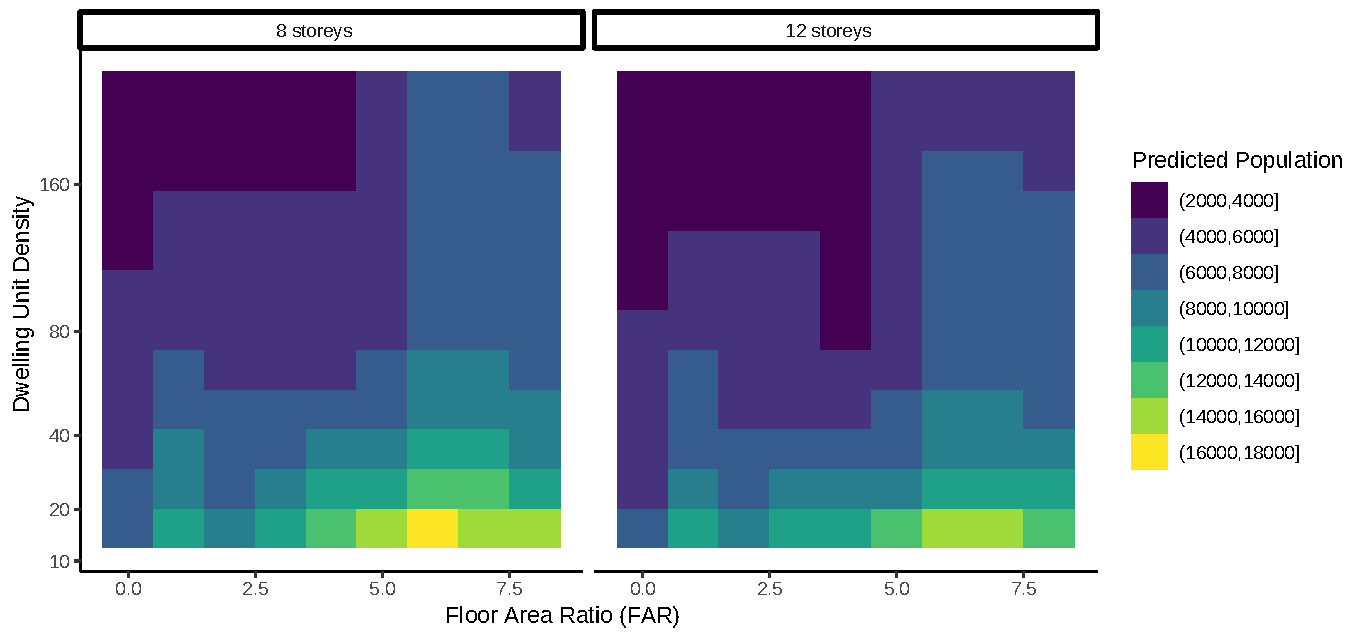
\includegraphics[width = \textwidth]{figuras/previsoes.pdf}
    \label{fig:previsoes}
\end{figure}

\subsection{Key results}

Despite the methodological differences, both approaches converge on a common result: housing density is the most important building pattern component in defining population density. This finding is intuitive, since the number of households plays a central role in determining the number of inhabitants. Building density and the number of floors, given a constant housing density and floors, can be seen as modifiers of the profile of these households.

As building density increases, housing units tend to be more spacious, which accommodates more residents on average. In the case of verticalization, with fixed building and housing density, any increase in floors requires a reduction in the land occupation rate (as discussed in Section \ref{sec:perg2} and Appendix \ref{appendix:verticalization}), resulting in buildings with larger setbacks. The data suggests that the same number of housing units and floor area, when inserted into more vertical developments, have fewer residents on average.

In light of the results presented, the discussion about the instruments established by the SMP takes a new turn. The data shows that verticalization, which was encouraged in the axis zones, is not an ally of densification, sometimes even working in the opposite direction. The effect of building density has been largely obstructed by the potential of housing density to generate density. In this sense, if the SMP aims to define which areas of the city should have higher or lower density, it would be more effective to focus on the land quota and allow a FAR and hight limit sufficient for the construction of housing units\footnote{A land quota of 20 means that, with the basic FAR, each housing unit will have 20 square meters. These same units with a FAR of 4 can have an average of 80$m^2$. However, it is impossible to achieve a FAR 4 with less than 4 floors. Even when there are obligatory setbacks, a greater number of floors than the FAR is necessary to be able to build all the square meters of floor area.}

\clearpage
\section{From regulation to building standards}
\label{sec:perg2}

The aim of this section is to answer: \textbf{Was regulation able to influence building standards in the city in the way expected?} To this end, two approaches were chosen. Both are, in essence, regression discontinuity methodologies (RDD\footnote{Regression Discontinuity Design}). This choice is ideal because of the exogeneity in which it was defined which plots would or would not belong to the axis areas near their border. As mentioned in Section \ref{sec:master-plan}, to become an axis zone, the plot must be within the area of influence of high-capacity public transport.

In this sense, the lots next to those classified as within the axis zone are a perfect control, since the difference between a treatment lot and a control lot is just crossing the street.

\begin{figure}[h]
    \centering
    \caption{Example of separation of control and treatment groups in Vila Mariana}
    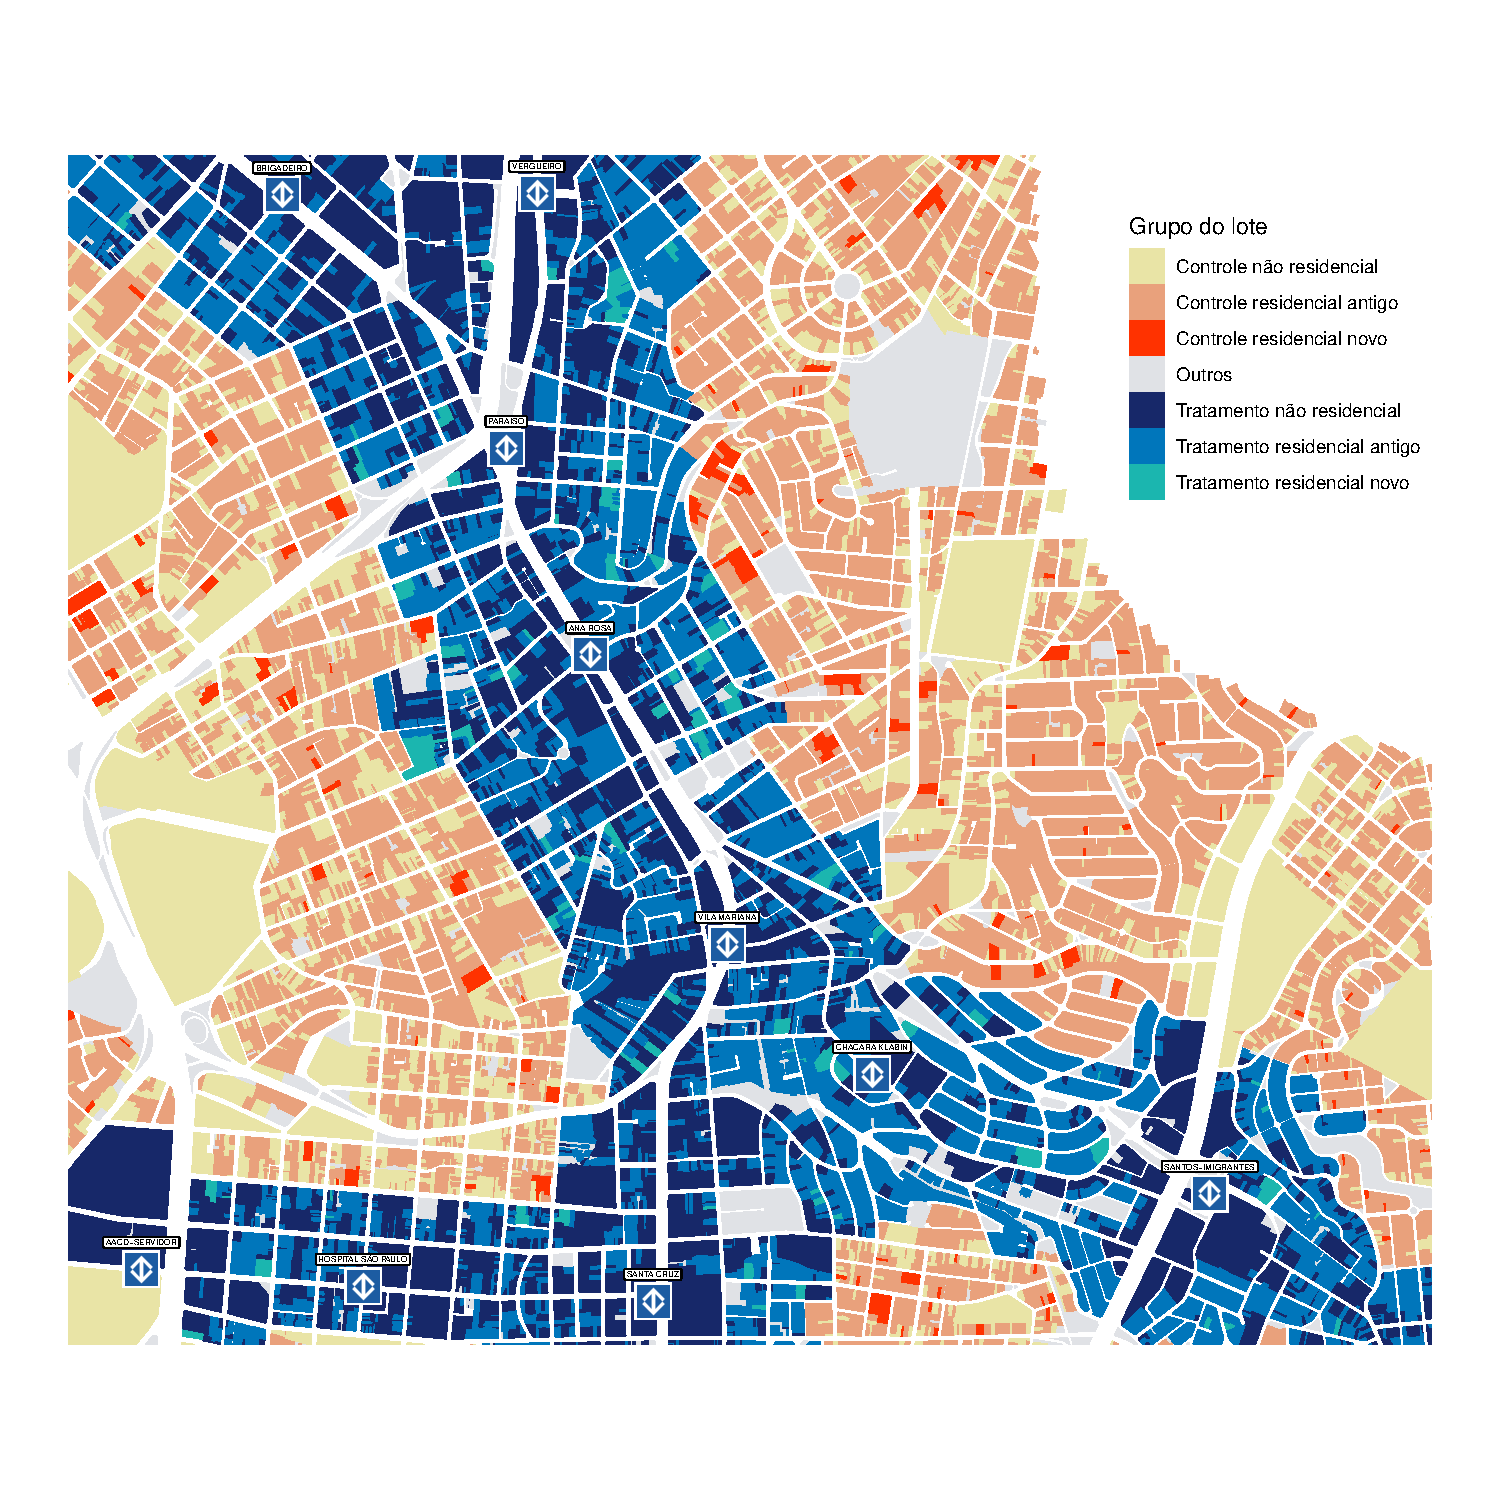
\includegraphics[width = .9\textwidth]{figuras/mapa-lotes-metro.pdf}
    \label{fig:mapaRDD}
\end{figure}

In Figure \ref{fig:mapaRDD} you can see an example of the classification of lots as control and treatment in Vila Mariana, a region of axes activated by metro stations, in a region where two lines join, the green and the blue. A development is considered new if it was completed after 2014, when the SMP came into effect.

Before moving on to causal inference, some interesting results can be obtained through descriptive statistics. Firstly, it is not possible to observe a large difference in the number of built-up plots between the control and treatment group after 2014 in Figure \ref{fig:delta-IPTU-lotes}. However, these plots now have a greater number of housing units, as illustrated in Figure \ref{fig:delta-IPTU-unidades}. This indicates an increase in housing density.  

\begin{figure}[h]
    \centering
    \caption{Change in the number of plots built on the border (50m) of the axes}
    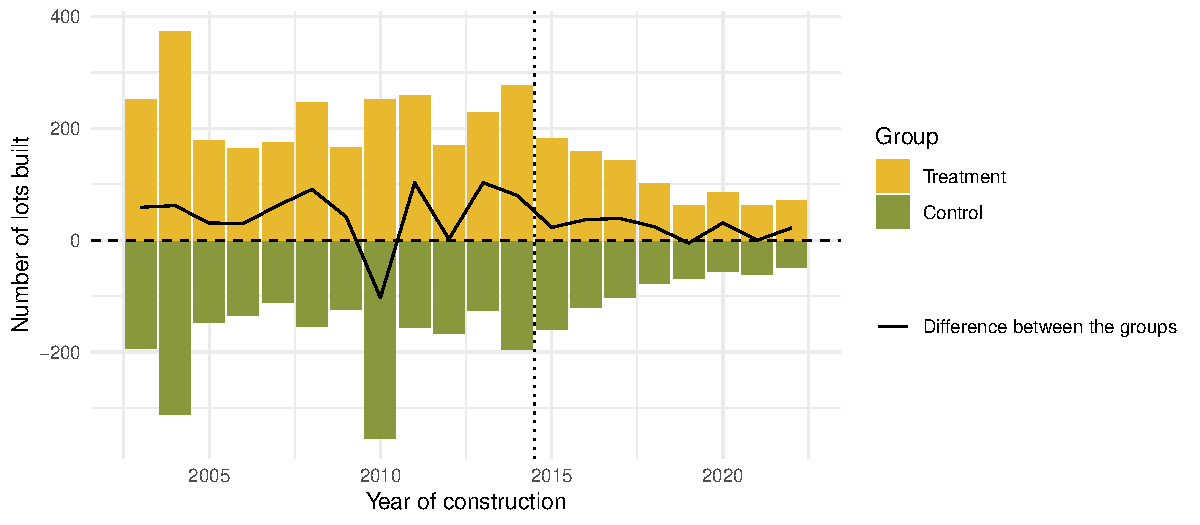
\includegraphics[width = .8\textwidth]{figuras/IPTU-delta-lotes.pdf}
    \label{fig:delta-IPTU-lotes}

    \caption{Change in the number of dwellings built on the border (50m) of the axes}
    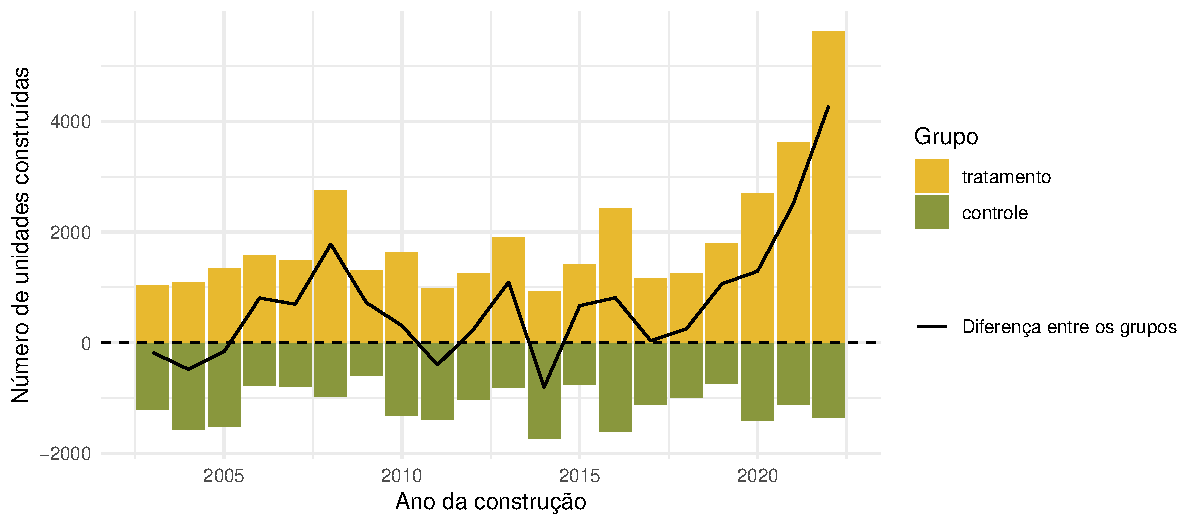
\includegraphics[width = .8\textwidth]{figuras/IPTU-delta-unidades.pdf}
    \label{fig:delta-IPTU-unidades}
\end{figure}

\subsection{Geographic \textit{diff-in-diff} approach (and \textit{event study})}
\label{subsec:perg2-did}
Geographical \textit{diff-in-diff (DiD)} is a category of difference-in-difference regression that takes into account the spatial proximity of observations when defining control and treatment criteria. In this case, all residential plots within a distance of 50m between the centroid and the edge of the axis were defined as treatment, and the same distance as control, but for plots outside the axis zone. The identification hypothesis is the same as for a common DiD: the two groups, in the absence of treatment, must show parallel trends.

\begin{table}[!t]
\caption{\label{tab:analise/did-IPTU}Resultados do DiD para unidades dentro de 50m da fronteira de eixo} 
\fontsize{12.0pt}{14.4pt}\selectfont
\begin{tabular*}{\linewidth}{@{\extracolsep{\fill}}lcccc}
\toprule
  & densidade\_construtiva & densidade\_habitacional & pavimentos & residencial \\ 
\midrule\addlinespace[2.5pt]
Intercepto & 1.031*** & 0.008*** & 1.992*** & 0.780*** \\ 
Tratamento & -0.001 & 0.000 & 0.027 & -0.011*** \\ 
Pós PDE & 0.891*** & 0.009*** & 1.661*** & -0.100*** \\ 
{Tratamento x Pós PDE} & {0.903***} & {0.011***} & {2.392***} & {0.001} \\ 
Num.Obs. & 59904 & 59904 & 59904 & 77625 \\ 
R2 & 0.027 & 0.032 & 0.026 & 0.001 \\ 
R2 Adj. & 0.027 & 0.032 & 0.026 & 0.001 \\ 
\bottomrule
\end{tabular*}
\begin{minipage}{\linewidth}
+ p < 0.1, * p < 0.05, ** p < 0.01, *** p < 0.001\\
\end{minipage}
\end{table}



Table \ref{tab:did-IPTU} shows the DiD results, choosing each component of the construction pattern as the variable of interest. The data shows that the introduction of the axes is responsible for increasing building density by an average of 0.9, housing density by 0.011 households per square meter of land and 2.4 floors. Furthermore, for this 50m section, there is no statistically significant difference between the control and treatment groups before the SMP. The results are robust to the different choices for the edge proximity cut-off. Figure \ref{fig:robustez-did-IPTU} in Appendix \ref{appendix:figures} shows the robustness of the results in relation to the choice of distance from the edge.

\begin{figure}[h]
    \centering
    \caption{\textit{Event study} for the construction patterns at the border (50m) of the axes}
    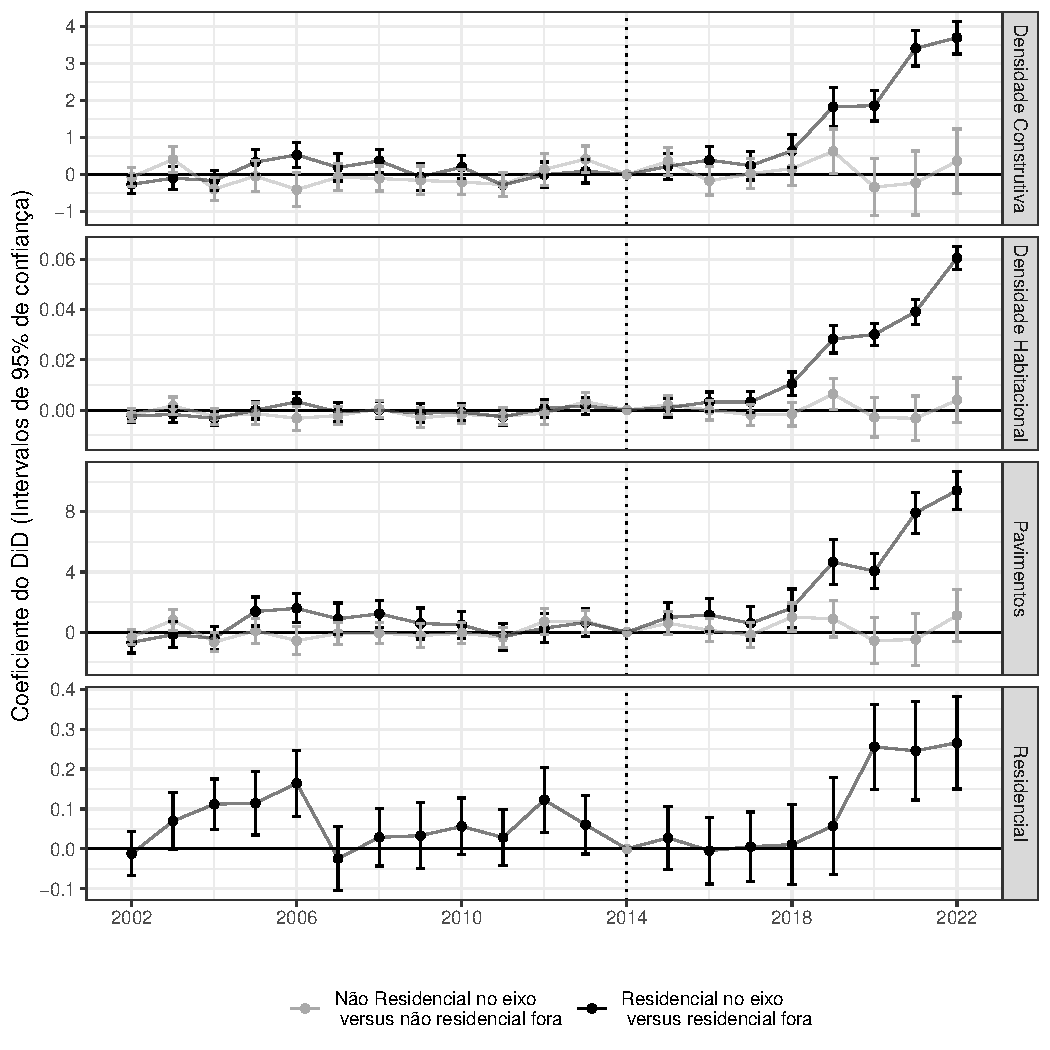
\includegraphics[width = .9\textwidth]{figuras/event-study.pdf}
    \label{fig:event-study}
\end{figure}

To strengthen the analysis and identify temporal heterogeneity in the results, an event study was also conducted with the same configurations. The results are presented in Figure \ref{fig:event-study}, in which each graph shows the regression whose variable of interest is indicated on the right-hand side. The \textit{event study} also points to an increase in building density, housing density and sidewalks after the SMP, but the effect seems to intensify after 2018. This can be explained by the fact that the developments delivered between 2014 and 2017 largely still followed the 2002 SMP regulations. In addition, parallel trends were observed in the pre-SMP period, indicating that the groups are in fact comparable and the criterion chosen for separating the groups is exogenous. Finally, a surprising result is that the axes only seem to have affected residential developments.

\subsection{RDD approach}

Assuming that plots that are close to the border of the axes are similar has succeeded in producing similar groups with parallel trajectories in Section \ref{subsec:perg2-did}, so using the RDD methodology may also be appropriate\footnote{Inclusive, RDD becomes the same as estimation by difference when the degree of the polynomial is equal to zero and the \textit{bandwidth} is the same}. The RDD identification hypothesis consists of considering that around the cut-off point, the observations immediately above and below the threshold are similar in all observable and unobservable characteristics, except for the treatment variable \cite{Cattaneo2019, Cattaneo2024}. As discussed at the beginning of Section \ref{sec:perg2}, this exogeneity exists, since the difference between a treatment batch and a control batch is just crossing the street.

\begin{figure}[!h]
    \centering

    \caption{RDD for building standards around the axes}
    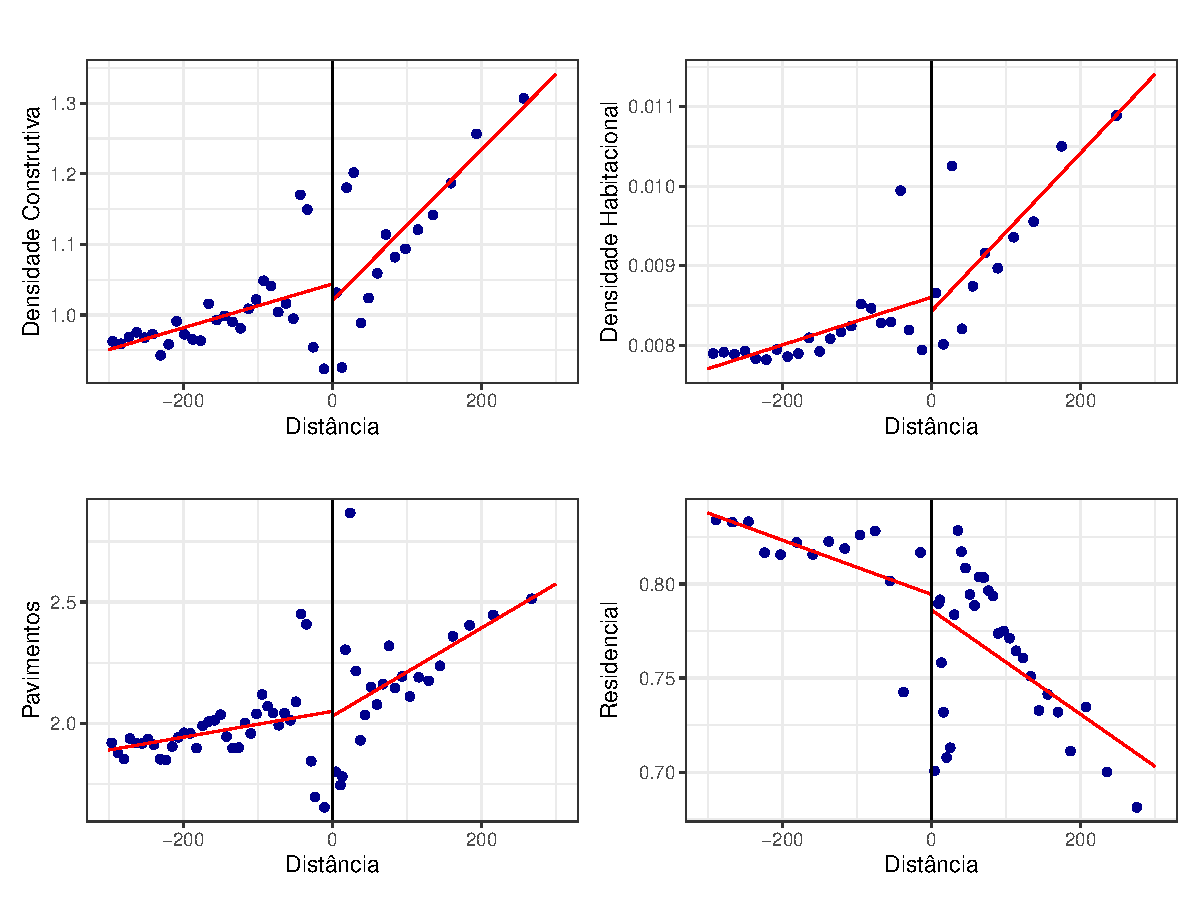
\includegraphics[width = .99\textwidth]{figuras/rdd-plot-IPTU.pdf}
    \label{fig:rdd-IPTU}

    \caption{RDD for building patterns around the axes, filtering by plots with buildings after 2014}
    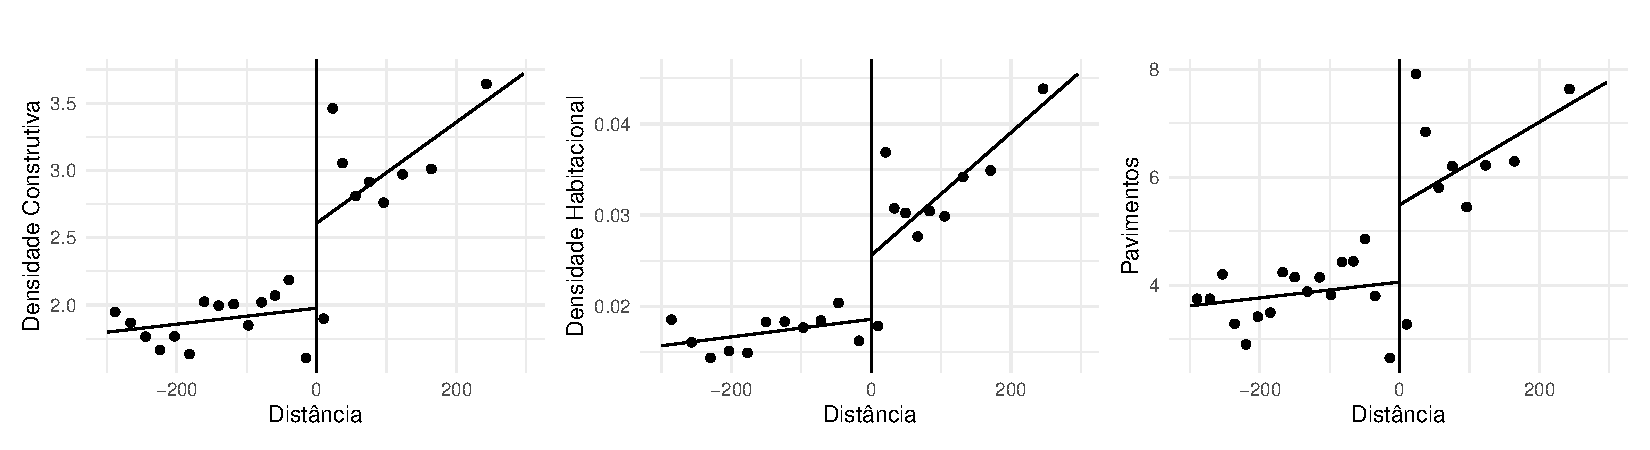
\includegraphics[width = .99\textwidth]{figuras/rdd-plot-IPTU-posPDE.pdf}
    \label{fig:rdd-IPTU-posSMP}
\end{figure}

However, when the RDD is implemented, there is no treatment effect - this result can be seen in Figure \ref{fig:rdd-IPTU}. The reason for this is that, as few plots have been built on since the SMP (see Figure \ref{fig:area-sector} and \ref{fig:delta-IPTU-lotes}), even if the effect is significant, it is imperceptible when all plots are considered. The result becomes significant when selecting only the plots that were built on after 2014. In this case, there is an increase in building density, housing density and floors (Figure \ref{fig:rdd-IPTU-posSMP}).

\begin{table}[h]
\centering
\caption{RDD results with only buildings from after the SMP (2014)} 
\fontsize{10pt}{12pt}\selectfont
\begin{tabular*}{.85\linewidth}{@{\extracolsep{\fill}}lccc}
\toprule
  & Densidade Construtiva & Densidade Habitacional & Pavimentos \\ 
\midrule\addlinespace[2.5pt]
Conventional & 0.707** & 0.010*** & 1.955** \\ 
Bias-Corrected & 0.638** & 0.010** & 1.821** \\ 
{Robust} & {0.638*} & {0.010*} & {1.821*} \\ 
\midrule
Observations (left)  & 622 & 799 & 624 \\ 
Observations (right) & 684 & 841 & 689 \\ 
Bandwidth & 61.2 & 76.3 & 61.7 \\ 
\bottomrule
\end{tabular*}
\begin{minipage}{.85\linewidth}
+ p < 0.1, * p < 0.05, ** p < 0.01, *** p < 0.001\\
\end{minipage}
\label{tab:rdd-IPTU}
\end{table}



\begin{table}[h]
  \centering
\caption{RDD placebo test with the cutoff 100 meters outside the axis region} 
\fontsize{10pt}{12pt}\selectfont
\begin{tabular*}{.85\linewidth}{@{\extracolsep{\fill}}lccc}
\toprule
  & Building Density & Dwelling Unit Density & Storeys \\ 
\midrule\addlinespace[2.5pt]
Conventional & 0.031 & 0.000 & 0.211 \\ 
Bias-Corrected & 0.096 & 0.001 & 0.407 \\ 
{Robust} & {0.096} & {0.001} & {0.407} \\ 
\midrule
Observations (left) & 863 & 921 & 890 \\ 
Observations (right) & 990 & 1070 & 1027 \\ 
Bandwidth & 76.9 & 82.7 & 79 \\ 
\bottomrule
\end{tabular*}
\begin{minipage}{.85\linewidth}
+ p < 0.1, * p < 0.05, ** p < 0.01, *** p < 0.001\\
\end{minipage}
\end{table}



Table \ref{tab:rdd-IPTU} shows the results of the RDD filtered only for lots with new buildings and using a triangular \textit{kernel} with an automatically chosen bandwidth. The results are similar to those found via differences in differences and those shown in Figure \ref{fig:rdd-IPTU-posSMP}. As a placebo test, the same procedure was replicated, but with the \textit{cutoff} set to -100 instead of zero. The automatically selected bandwidth was less than 100, which implies that in this procedure there was a comparison of the control group with the control group itself. The placebo test showed no effect for the three components of the constructive pattern, validating the test and providing further evidence for the exogeneity of the treatment at the border.

\subsection{Key results}

The data shows that buildings on the axes after the start of the SMP have higher building density, housing density and floor levels. The evidence also points to an intensification of the SMP effect starting in 2018 and reaching its peak in the most recent data, in 2022. In addition, the SMP changes seem to have only affected residential developments, while in other uses there is no significant difference between the on-axis and off-axis regions.

However, one result that also stands out is that the change caused by the SMP over the last 10 years has not been intense enough and/or fast enough to see a clear territorial division of axis and non-axis in construction patterns. In order to observe the results, it is necessary to look exclusively at new developments, which, as shown in Figure \ref{fig:area-sector}, represent less than 5\% of the built-up area within a 1km radius of the axis region.

\clearpage
\section{From regulation to population density}
\label{sec:perg3}

The aim of this section is to answer: \textbf{Has regulation been able to influence population density in the city?} As mentioned in Section \ref{sec:perg1}, housing density is the most important component in determining population density, and according to the results presented in Section \ref{sec:perg2} the axes caused an increase in housing density. Therefore, the hypothesis that makes the most sense is that the population density in the axes has increased. To test this hypothesis, we carried out a procedure similar to that presented in Section \ref{sec:perg2}, but changing the response variable to population density.

The main difference is that, in the case of density, the observation unit (census tract) is much larger geographically than the plots. It is therefore common for a census tract close to the border to occupy areas in both the control group and the treatment group, which requires its exclusion from the analysis. However, the occurrence of this phenomenon is so frequent that, in the immediate vicinity of the border, there is an insufficient number of units to carry out the analysis using RDD. This phenomenon is illustrated in Figure \ref{fig:rdd-density-census}.

In addition, there is a survival bias, in which only small census tracts, which are less likely to be on both sides of the border, remain close to the border after applying the exclusion criterion\footnote{In the case of the census tract, it is considered to be treated when its centroid is in the axis region and more than 95\% of its area is in this region. Control is defined by the presence of an off-axis centroid and less than 5\% of the axis area. Any census tract that does not meet one of the criteria is excluded}. The problem with these sectors is that, as discussed in Section \ref{sec:dataCensus}, the smaller the census sector, the higher its density tends to be, which causes the average density at the border to increase atypically in both the control and treatment groups. These factors make analysis via RDD unfeasible.

\begin{figure}[!h]
    \centering
    \caption{Number of observations per group as a function of distance from the axes boundary}
    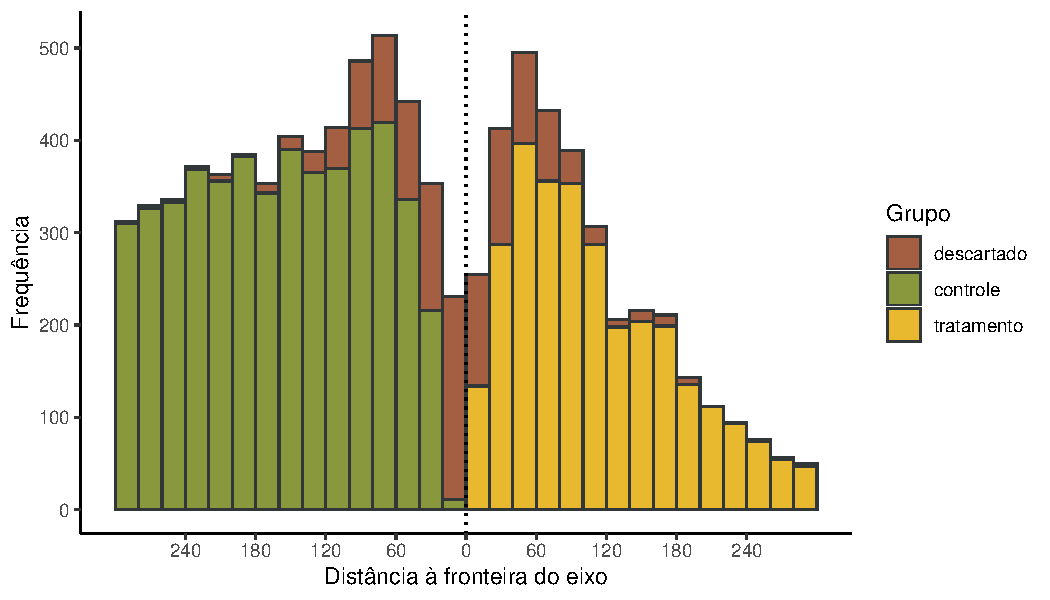
\includegraphics[width = .75\textwidth]{figuras/rdd-balanceamento-censo.pdf}
    \label{fig:rdd-density-census}
\end{figure}

As done in Section \ref{sec:perg2}, it is possible to obtain some preliminary results before building the regression models. By looking at the number of inhabitants on the border of the axis (50m away), it is possible to see, as shown in Table \ref{tab:censo-descritivo-fronteira}, that the treatment regions showed a higher population increase between 2010 and 2022. Although this result does not confer causal inference, it does support the hypothesis of densification as a result of regulation on the axes.

\begin{table}[h]
    \centering
    \caption{População antes e depois do PDE em cada grupo na fronteira do eixo (50m)}
    {\small
    \begin{tabular}{
        >{\raggedright\arraybackslash}p{0.1\linewidth} 
        >{\raggedleft\arraybackslash}p{0.125\linewidth} 
        >{\raggedleft\arraybackslash}p{0.125\linewidth} 
        >{\raggedleft\arraybackslash}p{0.125\linewidth}}
        % \toprule
        \textbf{Grupo} & \textbf{2010} & \textbf{2022} & \textbf{$\Delta$} \\
        \midrule
        Tratamento & 92.964 & 133.898 & 40.934 \\
        Controle & 56.816 & 84.315 & 27.499 \\
    \end{tabular}
    }
    \label{tab:censo-descritivo-fronteira}
\end{table}

When analyzing the population growth of the entire axis region, a different picture emerges. The main advantage of comparing areas close to the border, as shown in Table \ref{tab:censo-descritivo-fronteira}, lies in the greater comparability between the groups, which share practically all the relevant characteristics - such as proximity to economic and mobility opportunities - with the exception of the urban regulation to which they are subject. However, when we expand the analysis to the entire axis region and contrast it with the rest of the city, we see a population variation that is contrary to what we would expect. As illustrated in Figure \ref{tab:censo-descritivo}, while the population of the city outside the axes registered an increase of approximately 400,000 inhabitants, the region around the axes paradoxically showed a decline in the number of residents.

\begin{table}[h]
    \centering
    \caption{Population before and after the SMP in each part of the city}
    {\small
    \begin{tabular}{
        >{\raggedright\arraybackslash}p{0.15\linewidth} 
        >{\raggedleft\arraybackslash}p{0.15\linewidth} 
        >{\raggedleft\arraybackslash}p{0.15\linewidth} 
        >{\raggedleft\arraybackslash}p{0.15\linewidth}}
        % \toprule
        \textbf{Region} & \textbf{2010} & \textbf{2022} & \textbf{$\Delta$} \\
        \midrule
        Outside axis & 9.795.114 & 10.192.905 & +397.791 \\
        Inside axis & 1.414.559 & 1.259.094 & -155.465 \\
    \end{tabular}
    }
    \label{tab:censo-descritivo}
\end{table}

However, it is important to note that these results are purely descriptive and it is not possible to say that the regulation of the axes was responsible for this change. Various factors unrelated to the master plan may have influenced citizens' choice of location. Section \ref{subsec:perg3did} presents an analysis that seeks to find a causal effect for the effect of regulation on population density.

\subsection{Differences-in-differences approach}
\label{subsec:perg3did}

The identification strategy remains the same as in Section \ref{sec:perg2}, in which only census tracts close to the border of the axis were considered, where the difference between control and treatment is just crossing the street. Based on this, a \textit{diff-in-diff} was conducted with a fixed effect for year and also with a fixed effect for census tract. The results can be seen in Table \ref{tab:did-censo}. The regressions in columns (A) and (C) present \textit{pooled} data with only year and group fixed effects, while in columns (B) and (D) they are panel regressions with both year and census sector fixed effects. Approximately 90\% of the census tracts analyzed in the region change position and/or size between 2010 and 2022, but the 10\% that maintain the same shape can be compared in time\footnote{While the 2010 Census had 18,953 census tracts, the 2022 Census has 27,592, which implies that the grid has changed significantly}, making panel analysis possible.

\begin{table}[!t]
\caption{Resultado diff-in-diff do Censo, para setores censitários em um raio de 100m dos eixos} 
\centering
\fontsize{12.0pt}{14.4pt}\selectfont
\begin{tabular*}{.7\linewidth}{@{\extracolsep{\fill}}lcc}
  & (A) & (B) \\ 
\midrule\addlinespace[2.5pt]
Intercepto & 0.057*** & 0.050*** \\ 
T (Grupo de tratamento) & -0.003 & 0.000 \\ 
P (Período pós PDE) & -0.015*** & -0.011** \\ 
Q (Percentual residencial novo) &  & 0.108*** \\ 
T x P & -0.001 & -0.004 \\ 
T x Q &  & -0.055* \\ 
P x Q &  & -0.045* \\ 
{T x P x Q} & {} & {0.043} \\ 
\midrule
Num.Obs. & 3217 & 3217 \\ 
R2 & 0.013 & 0.040 \\ 
R2 Adj. & 0.012 & 0.037 \\ 
\bottomrule
\label{tab:did-censo}
\end{tabular*}
\begin{minipage}{.7\linewidth}
+ p < 0.1, * p < 0.05, ** p < 0.01, *** p < 0.001\\
\end{minipage}
\end{table}



The evidence shown in Table \ref{tab:did-censo} points to an increase in population density as a result of the regulation of the axes, despite the significance of only 5\% (Columns A, B and D). However, it is important to note that this effect was estimated locally and cannot be extrapolated to the core of the axes or to the rest of the city. The results are robust to different distance cut-offs, if the census sector fixed effect is incorporated at a significance level of 5\%. There is no distance cut-off that points to 1\% statistical significance of the coefficient associated with the treatment. The regression coefficients can be analyzed in Figure \ref{fig:robustez-did-censo} of Appendix \ref{appendix:robustness} for different distance cut-offs.

\subsection{Key results}


The results indicate that the population density on the transportation axes increased after the implementation of the SMP, when compared to the immediately adjacent regions. This result has a significance level of 5\% and is largely consistent for different proximity cut-offs. On the other hand, as shown in Table \ref{tab:censo-descritivo}, the total population in the axis region did not increase between 2010 and 2022, as expected with the SMP. Thus, even if the SMP has had a positive effect on population densification, the result after 10 years of the plan's validity is still not enough to see a large portion of the population beginning to inhabit the axes.


\chapter{Conclusion}
\label{chp:conclusion}

\section{Key results}
\label{sec:conclusion}

Based on the results obtained, it was possible to break down the analysis into three fundamental aspects, as shown in Figure \ref{fig:diagram}: (i) the relationship between regulatory instruments and building standards, (ii) the effectiveness of these standards in generating the expected population density and (iii) the final relationship between regulation and population density.

Firstly, the regulatory instruments introduced by the 2014 master plan proved to be effective in changing the construction standards of the new plots built in the axis. The difference-in-differences (DiD) analysis revealed that after the implementation of the SMP, especially from 2018 onwards, the transportation axes attracted developments with higher building density, housing density and floors per building. Discontinuity regression (RDD) complements these findings with similar estimates. These results suggest that urban regulation in the axes acted as expected in terms of changing building patterns. However, the speed at which this change occurs has not yet been sufficient to observe a spatial discontinuity at the border of the axes\footnote{if the information on the year in which the plot was built was hidden, it would not be possible to find out, just by looking at the building patterns, where the border of the axis is in most of the city}.

Secondly, when evaluating the capacity of these building standards to generate the expected population density, the results highlighted housing density as the main determinant of population density. The analysis shows that the land quota - responsible for defining a minimum number of housing units - has a more direct influence on the increase in residents in the axis areas than the FAR and hight limit instruments. In contrast, verticalization showed a negative relationship with population density when building and housing density are kept constant, highlighting the association between vertical developments and smaller family nuclei.

Finally, by connecting the dots and looking at the impact of regulation on population density in the axis, the evidence suggests that the policy implemented by the SMP has indeed resulted in an increase in population occupation in these areas. On the other hand, even if the SMP has had a positive effect on population densification, the result after 10 years of the plan's validity is still not enough to see a large portion of the population beginning to inhabit the axes. Even so, the SMP, through its regulatory instruments, has managed to direct population densification, albeit with moderate intensity, towards the areas surrounding high-capacity public transport, which was its main objective.  

\section{Main limitations}

In addition, the census tract mesh does not remain the same from one year to the next, making it difficult to track census tracts over time. In the analysis conducted, only around 10\% of the census sectors in the area of interest did not change shape and could be monitored between 2010 and 2022.

The main limitation of the research is the level of observation of the Census data. Although the Census is commonly analyzed using micro-data, in which each observation represents an individual, the approach adopted in this research requires the use of georeferenced data. To do this, it is necessary to work at the census tract scale, which is the most disaggregated level available for georeferenced Census data. However, census tracts aggregate information on hundreds of individuals, which significantly reduces the granularity of the analysis.

This limitation is particularly relevant for this study due to the large geographical extent of many census tracts. Often, the same sector includes areas that received the treatment and others belonging to the control region, making it difficult to accurately identify the effects of the SMP. In the analysis conducted in Section \ref{sec:perg3}, it was found that, in 2022, 504,517 inhabitants lived in census tracts that had to be excluded from the analysis because of this overlap. The number of inhabitants remaining in the treatment group - sectors completely within the axis areas - was 680,616. This substantial reduction in sample size represents a major source of loss in the statistical power of the tests.

In addition, the grid of census tracts changes over time, making it difficult to follow the units of analysis over time. In the case of this study, only around 10\% of the census tracts located in the area of interest kept their shape unchanged between 2010 and 2022, making it impossible to carry out a consistent analysis over time. This discontinuity represents yet another methodological barrier, compromising comparability between the periods analyzed.


\section{Contributions to the public debate}
\label{sec:contributions}

Although the SMP has contributed to densification in the axis areas, it is essential to highlight the strengths and limitations of the mechanisms used. The SMP is expected to be in force until 2029, so bringing evidence to the public debate is of paramount importance so that the decisions that will be made for the 2030 SMP are based on facts.

Among the successes, based on the results presented, the introduction of the quota share was decisive for the success of densification in the axes, arousing interest in understanding how to optimize the use of this instrument. In the 2014 SMP, only the axis regions had the land quota regulated, while the rest of the city was left without maximum limits - a decision that could be reconsidered, given the effectiveness of the instrument. In addition, it is important to investigate whether the value of 20 is really ideal for the quota share in the axis areas.

On the other hand, the revision of the SMP in 2023 introduced a significant change to the quota share rule, allowing it to be made more flexible by applying the \textit{Social Factor} -- a multiplier on the value of the onerous grant. In practice, companies can pay more tax to exceed the limits of the regulated quota share. This measure runs counter to the central objectives of the SMP, as it weakens the main instrument responsible for directing population density towards the hub regions.

Another important aspect is the decision to remove the height limits. Although this choice seeks to encourage densification, the data suggests that, for a given floor area ratio (FAR) and land quota, more vertical developments tend to house fewer residents on average. This is because, when fixing the number of housing units and floor area, increasing the height of buildings is associated with greater setbacks and lower land occupation rates - in practice, this construction pattern is associated with housing with fewer inhabitants. In this sense, removing the height limits was a mistake.

Finally, it's important to note that the effect of the SMP was not exactly to encourage densification, but only to allow it to occur. For example, the FAR allowed on the axes was set between 2 and 4, but within this range there are no clear incentives to reach values close to the ceiling -- the same problem applies to the land quota. The peculiarity of this system of limitations rather than incentives comes from the real estate market's response to the rules of the game. In this sense, the SMP did not give the market reasons to densify, but allowed densification that was repressed by the old rules to become possible in the regions it chose.

